% !TeX encoding = UTF-8
% !TeX spellcheck = en_US

\documentclass[32pt,t]{beamer}
	\usepackage[utf8]{inputenc} % Sonderzeichen
	\usepackage[english]{babel}
	\usepackage{graphicx} % Bilder
	\usepackage{hyperref} % Hyperlinks
	\usepackage{graphicx} % Bilder

	\usepackage{amsmath} % Mathe, lädt amsmath gleich mit
	\usepackage{amssymb} % Mathesymbole
	\usepackage{amsthm} % Theorem-Umgebungen
	\usepackage{todonotes}
	\usepackage{subfig}
	\usepackage{tikz} % für Graphen, Automaten etc.
	
	\mode<presentation>
	\usetheme{Madrid}
	\usecolortheme[named=blue]{structure}
	\usefonttheme[onlymath]{serif}
	\useinnertheme{circles}
	\useoutertheme{infolines}
	\setbeamertemplate{blocks}[rounded][shadow=true]
	\usepackage{pifont}
	
	%remove default navigation in the bottom right corner
	\beamertemplatenavigationsymbolsempty
				
%Einstellungen
	\hypersetup{
		pdftitle = {Transforming Constraints to Application Conditions - Presentation 06/02/2017},
	} 

% Inhalt des Dokumentes
\begin{document}
	\title{From Constraints to Application Conditions}
	\subtitle{Presentation}
	\date{06/02/2017}
	\author{Robin Oppermann and Patrick Robrecht}
	
	\begin{frame}
		\titlepage
		
		\begin{center}
			Fundamentals of Model-Driven Engineering \\
			Jun.-Prof. Anthony Anjorin \\
			Research Group Database and Information Systems \\
			Department of Computer Science \\
			Paderborn University
		\end{center}
	\end{frame}

\section{Introduction}
	\begin{frame}
		\frametitle{Introduction}
		\framesubtitle{Constraint Example: Each List $J$ with a card $X$ has a previous list $K$}
		\centering
		\includegraphics[width=\linewidth]{Images/01_Constraint_Example}
	\end{frame}

	\begin{frame}
		\frametitle{Introduction}
		\framesubtitle{Rule Example: Moving Card $C$ from List $L$ to $L'$}
		\centering
		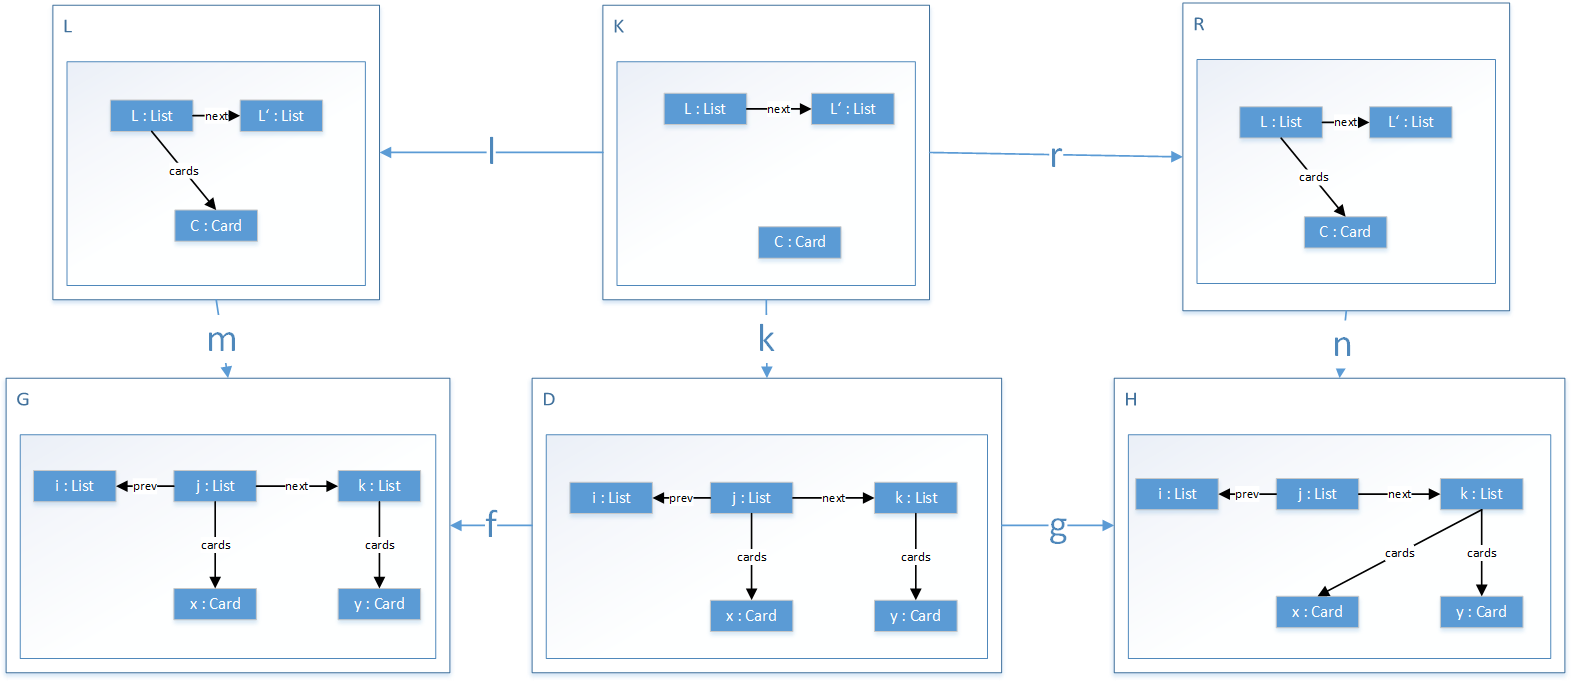
\includegraphics[width=\linewidth]{Images/01_Rule_Example}
	\end{frame}

	\begin{frame}
		\frametitle{Introduction}
		\framesubtitle{Why do we want to construct application conditions from constraints?}		
		\begin{itemize}
			\item model transformation system containing sets of rules and constraints
			\item need to ensure: graph after rule application does not violate a constraint
			\item idea: construct application conditions to check this before rule application
			\item regeneration after changes in rules / constraints necessary \\
			$\Rightarrow$ construction needs to be automatized 
		\end{itemize}
	\end{frame}
	
	\begin{frame}
		\frametitle{Contents}
		\tableofcontents
	\end{frame}

\section{Construction of Right Application Conditions from Constraints}
	\begin{frame}
		\frametitle{Contents}
		\tableofcontents[currentsection]
	\end{frame}

	\begin{frame}
		\frametitle{Construction of Application Conditions from Constraints}
		\framesubtitle{Construct possible epimorphic gluings $S$ -- Schema}
		\centering
		\includegraphics[width=\linewidth]{Images/10_Construct_S_Schema}
	\end{frame}

	\begin{frame}
		\frametitle{Construction of Application Conditions from Constraints}
		\framesubtitle{Construct possible epimorphic gluings $S$ -- Example Step 1}
		\centering
		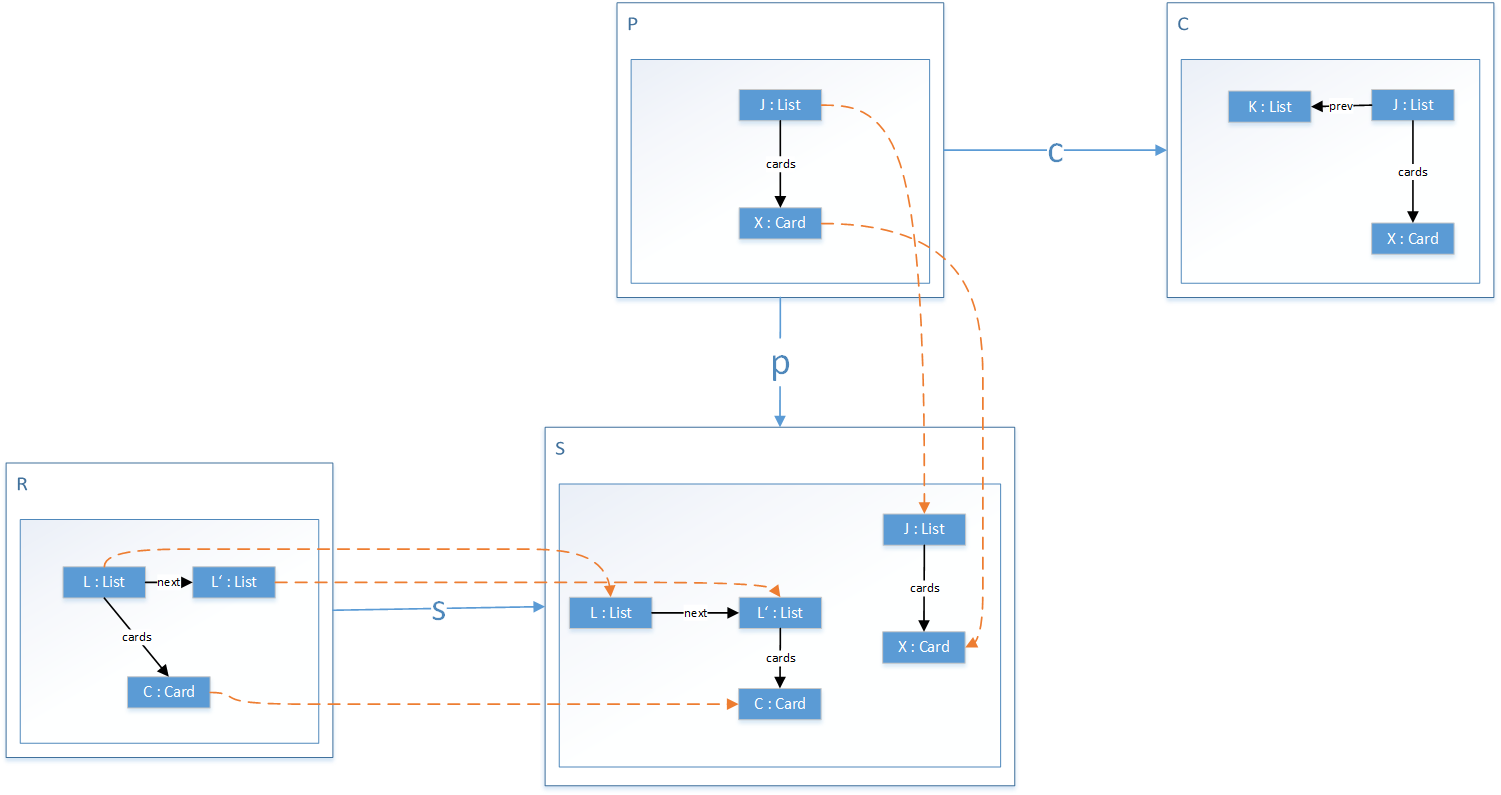
\includegraphics[width=\linewidth]{Images/11_Construct_S_Example_Step1}
	\end{frame}
	
	\begin{frame}
		\frametitle{Construction of Application Conditions from Constraints}
		\framesubtitle{Construct possible epimorphic gluings $S$ -- Example Step 2}
		\centering
		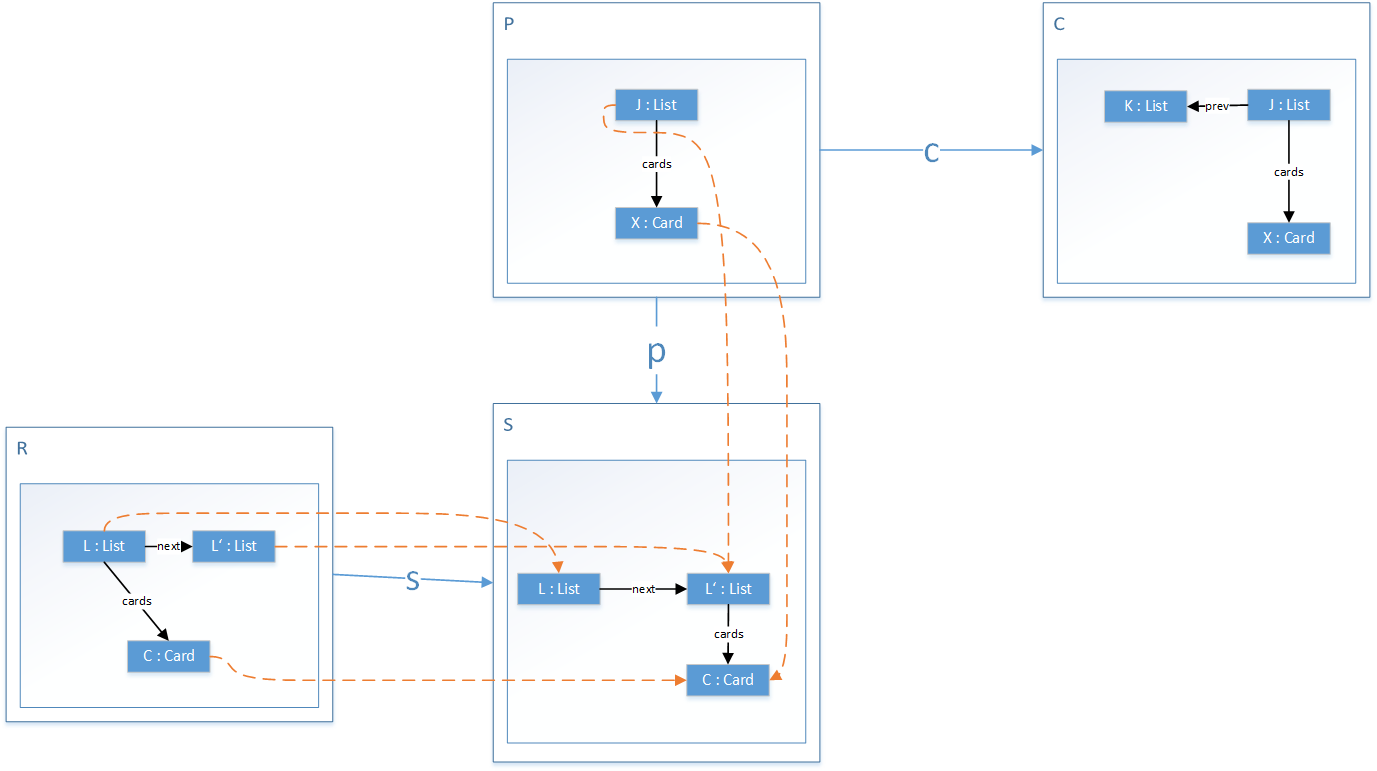
\includegraphics[width=\linewidth]{Images/12_Construct_S_Example_Step2}
	\end{frame}

	\begin{frame}
		\frametitle{Construction of Application Conditions from Constraints}
		\framesubtitle{Construct pushout $T$ -- Schema}
		\centering
		\includegraphics[width=\linewidth]{Images/20_Construct_T_Schema}
	\end{frame}

	\begin{frame}
		\frametitle{Construction of Application Conditions from Constraints}
		\framesubtitle{Construct pushout $T$ -- Example}
		\centering
		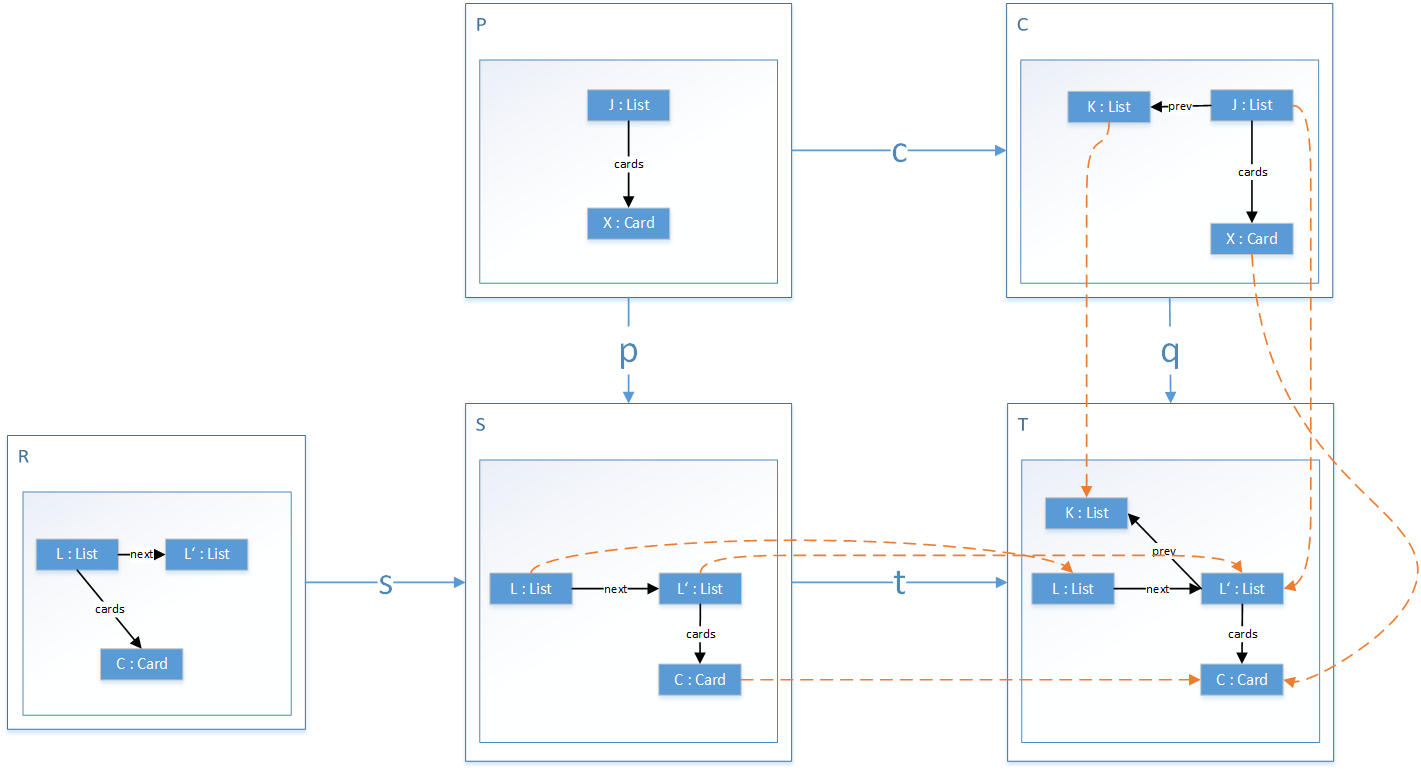
\includegraphics[width=\linewidth]{Images/21_Construct_T_Example}
	\end{frame}

	\begin{frame}
		\frametitle{Construction of Application Conditions from Constraints}
		\framesubtitle{Construct epimorphic gluings $T_i$ -- Schema}
		\centering
		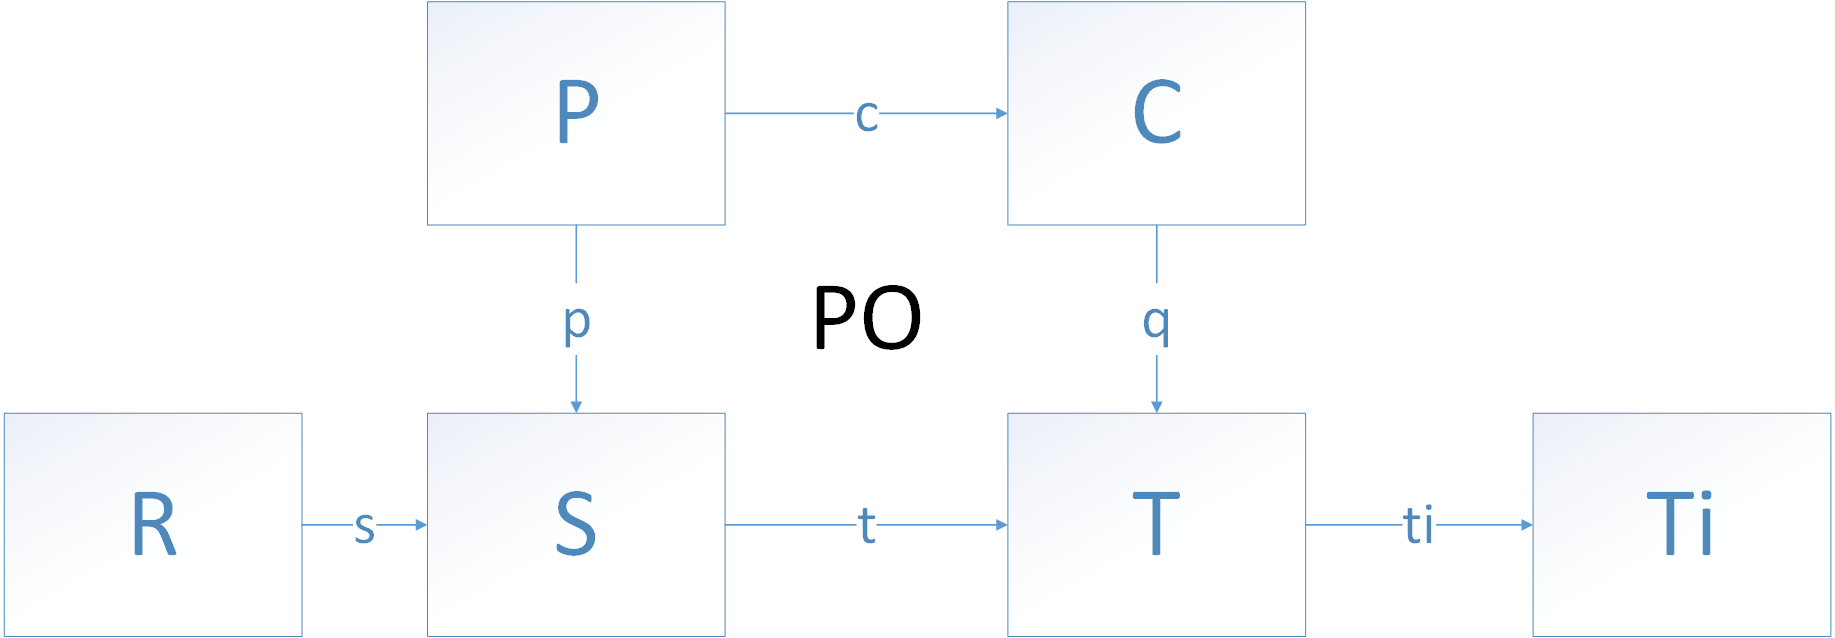
\includegraphics[width=\linewidth]{Images/30_Construct_Tis_Schema}
	\end{frame}

	\begin{frame}
		\frametitle{Construction of Application Conditions from Constraints}
		\framesubtitle{Construct epimorphic gluings $T_i$ -- Example}
		\centering
		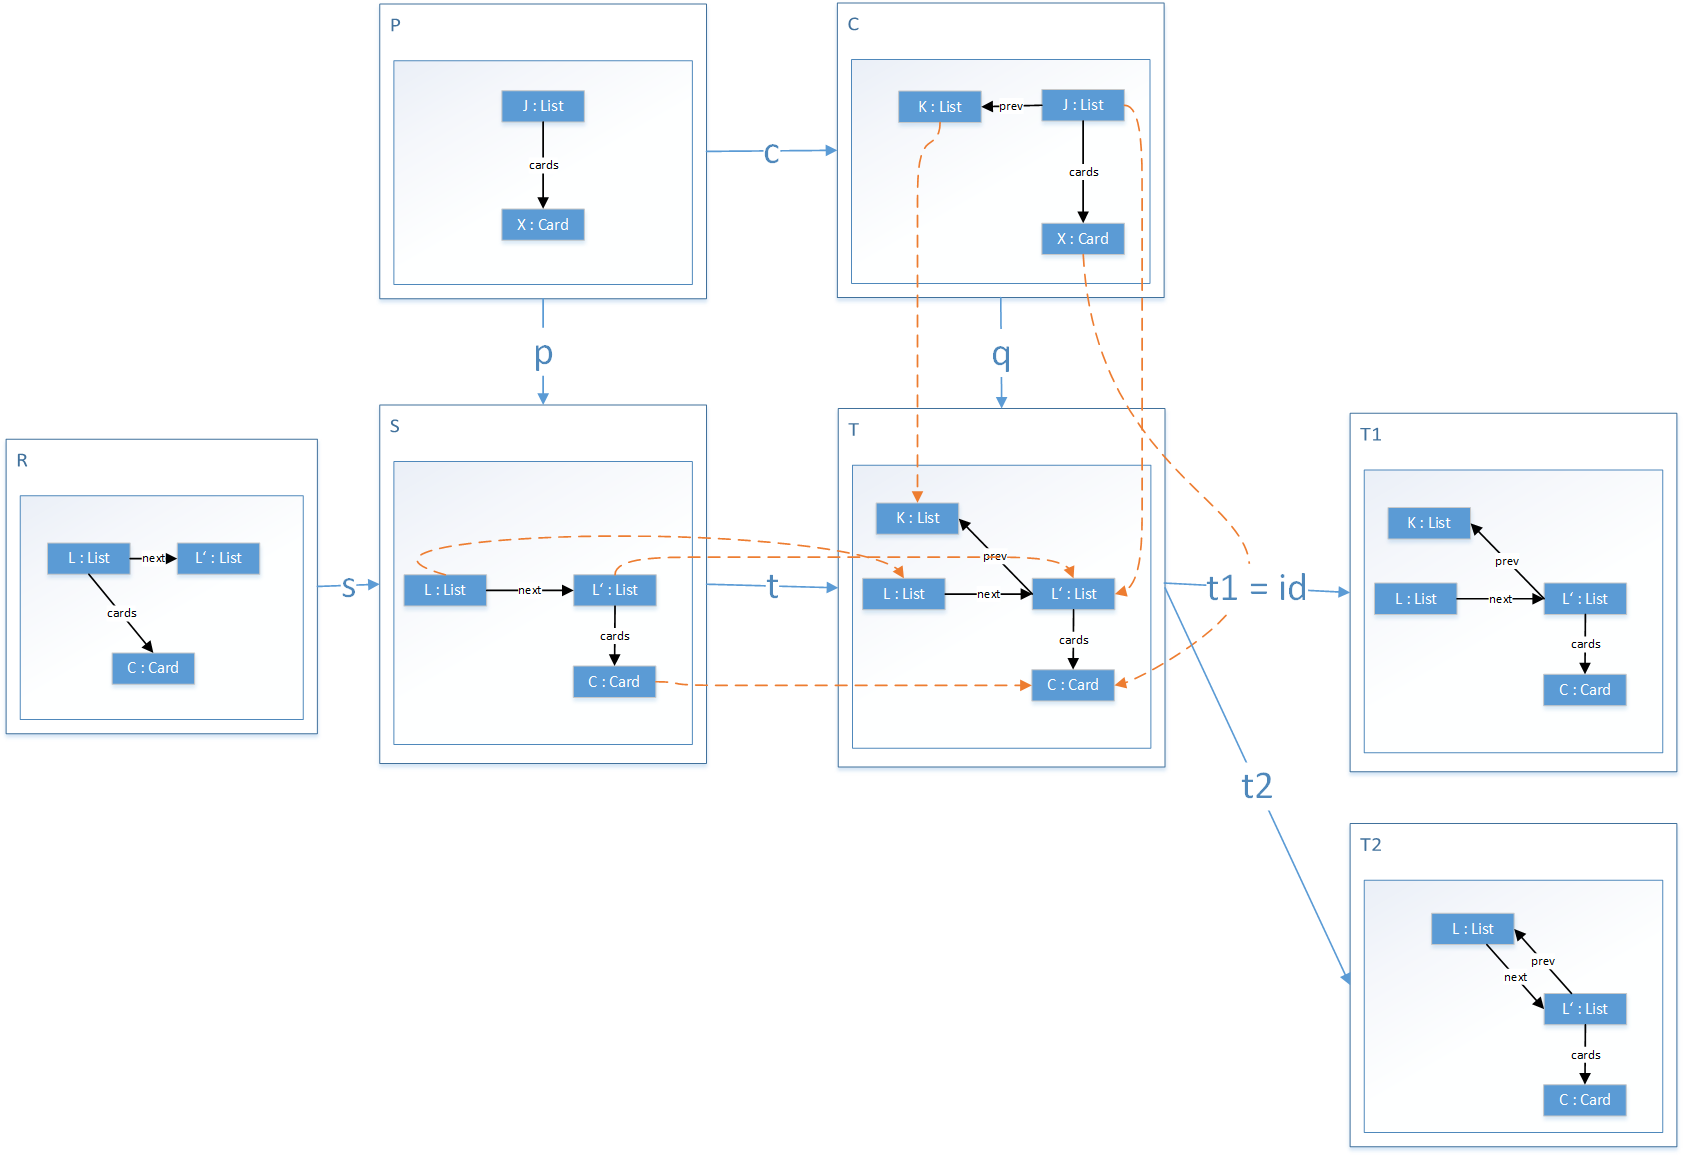
\includegraphics[height=.8\textheight]{Images/31_Construct_Tis_Example}
	\end{frame}

\section{Construction of Left from Right Application Conditions}
	\begin{frame}
		\frametitle{Contents}
		\tableofcontents[currentsection]
	\end{frame}

	\begin{frame}
		\frametitle{Construction of Left from Right Application Conditions}
		\framesubtitle{What we have done so far: Right Application Conditions}
		\centering
		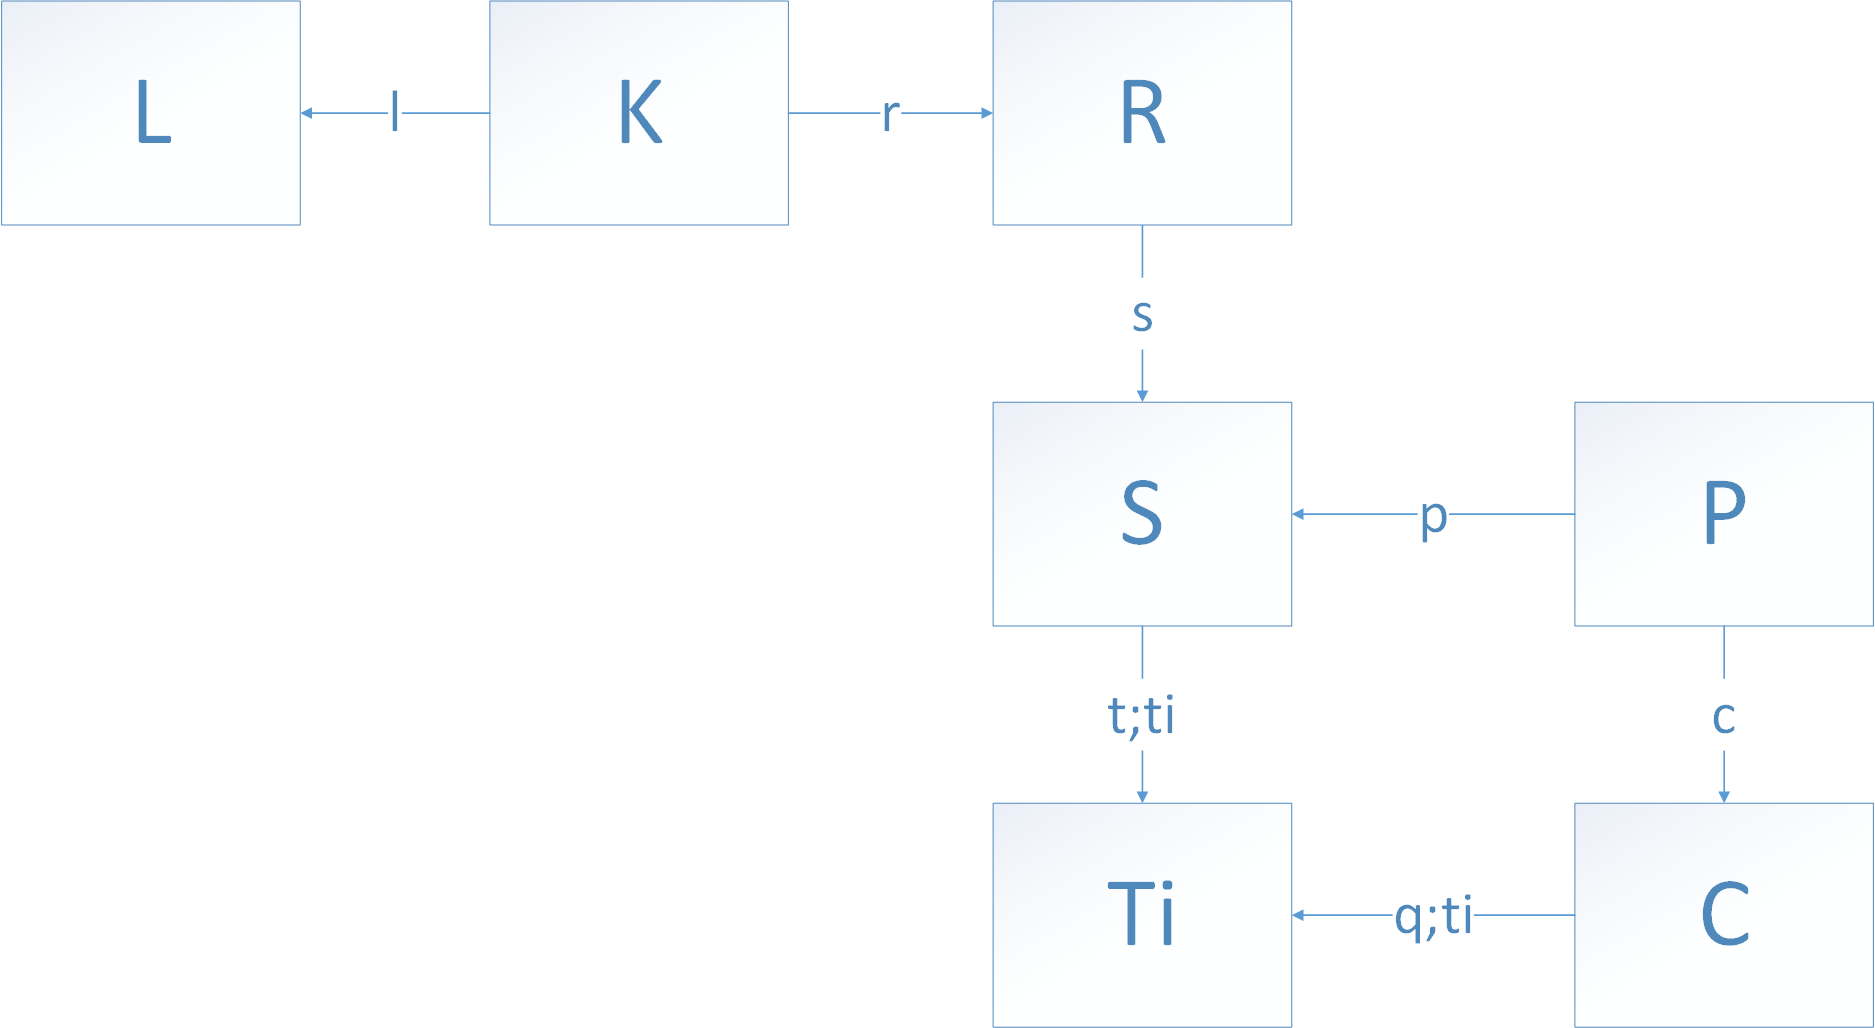
\includegraphics[width=\linewidth]{Images/40_Overview_RightAC_Schema}
	\end{frame}

	\begin{frame}
		\frametitle{Construction of Left from Right Application Conditions}
		\framesubtitle{Right Application Condition -- Example}
		\centering
		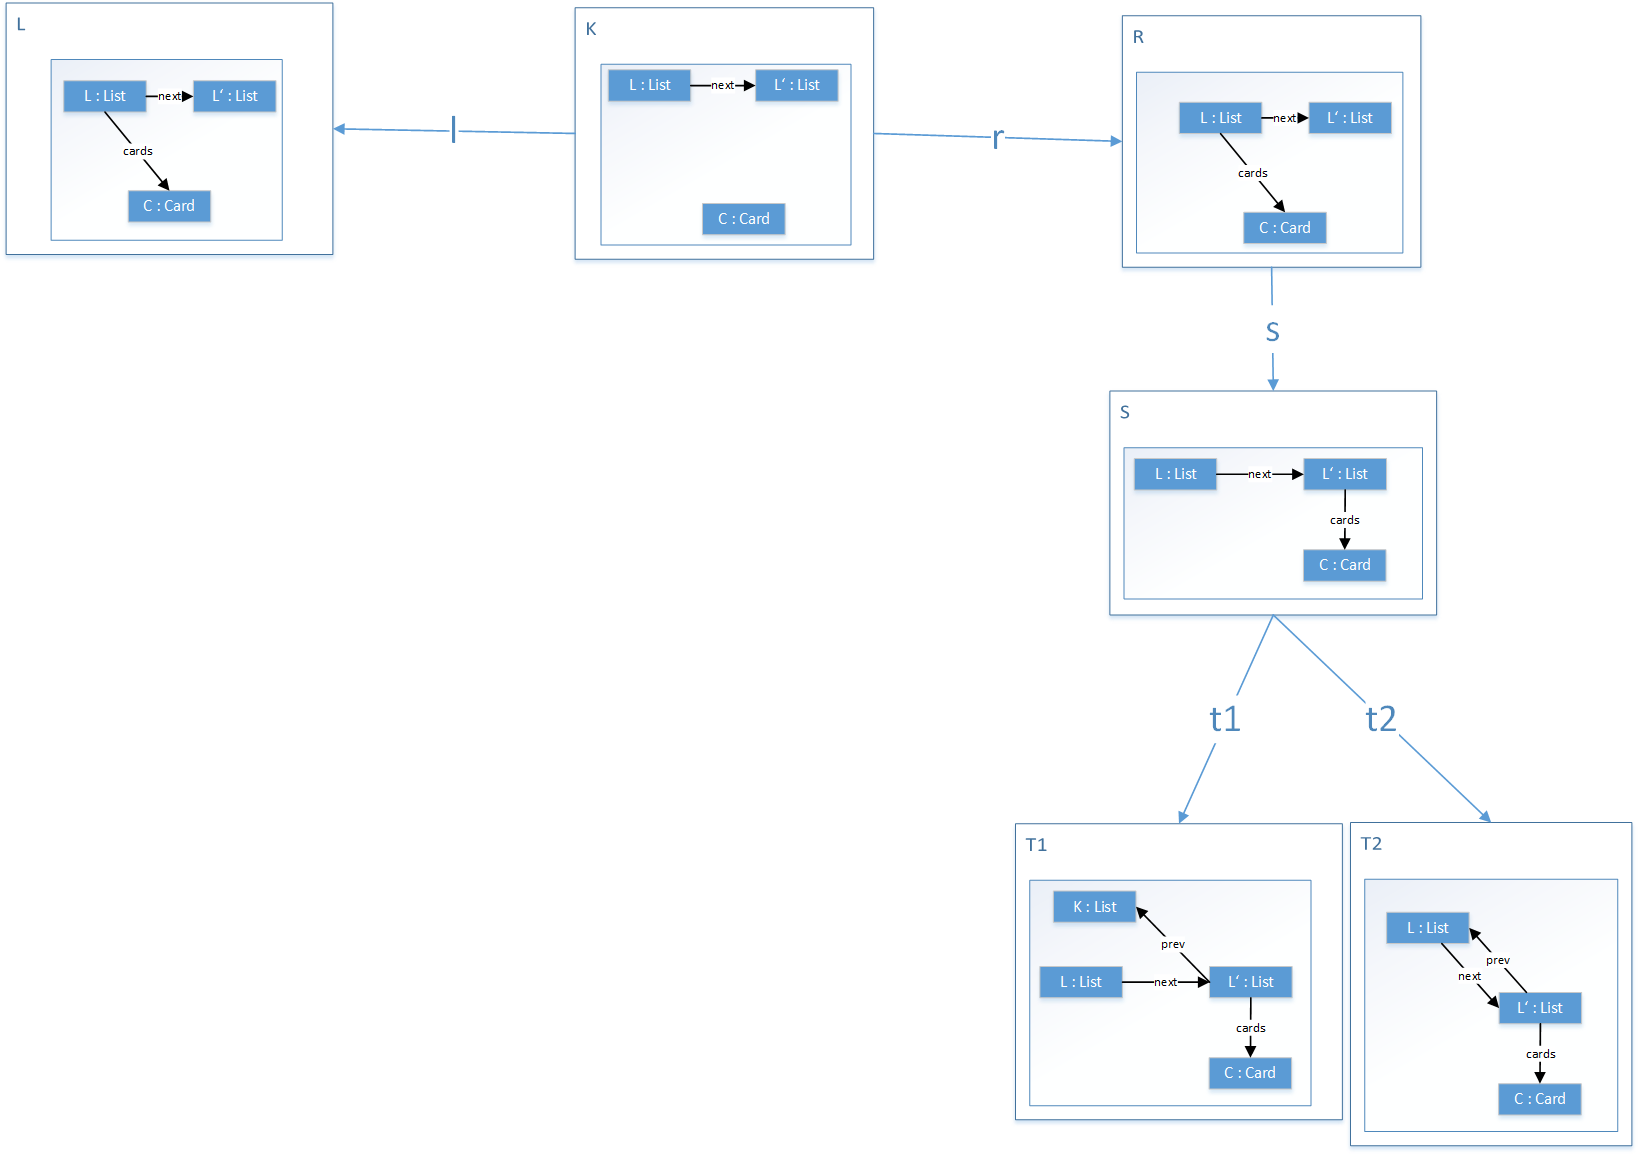
\includegraphics[height=.8\textheight]{Images/51_RightAC-To-LeftAC_Example_Step1}
	\end{frame}

	\begin{frame}
		\frametitle{Construction of Left from Right Application Conditions}
		\framesubtitle{Left and Right Application Conditions}
		\begin{block}{Right application condition}
			Rule is applicable if the right application condition holds in $H$ (i. e. after rule application).
		\end{block}
		\begin{block}{Left application condition}
			Rule is applicable if the left application condition holds in $G$ (i. e. before rule application), so the application of the rule doesn't result in a graph violating one of the constraints.
		\end{block}
	\end{frame}

	\begin{frame}
		\frametitle{Construction of Left from Right Application Conditions}
		\framesubtitle{From Right to Left Application Conditions -- Schema}
		\centering
		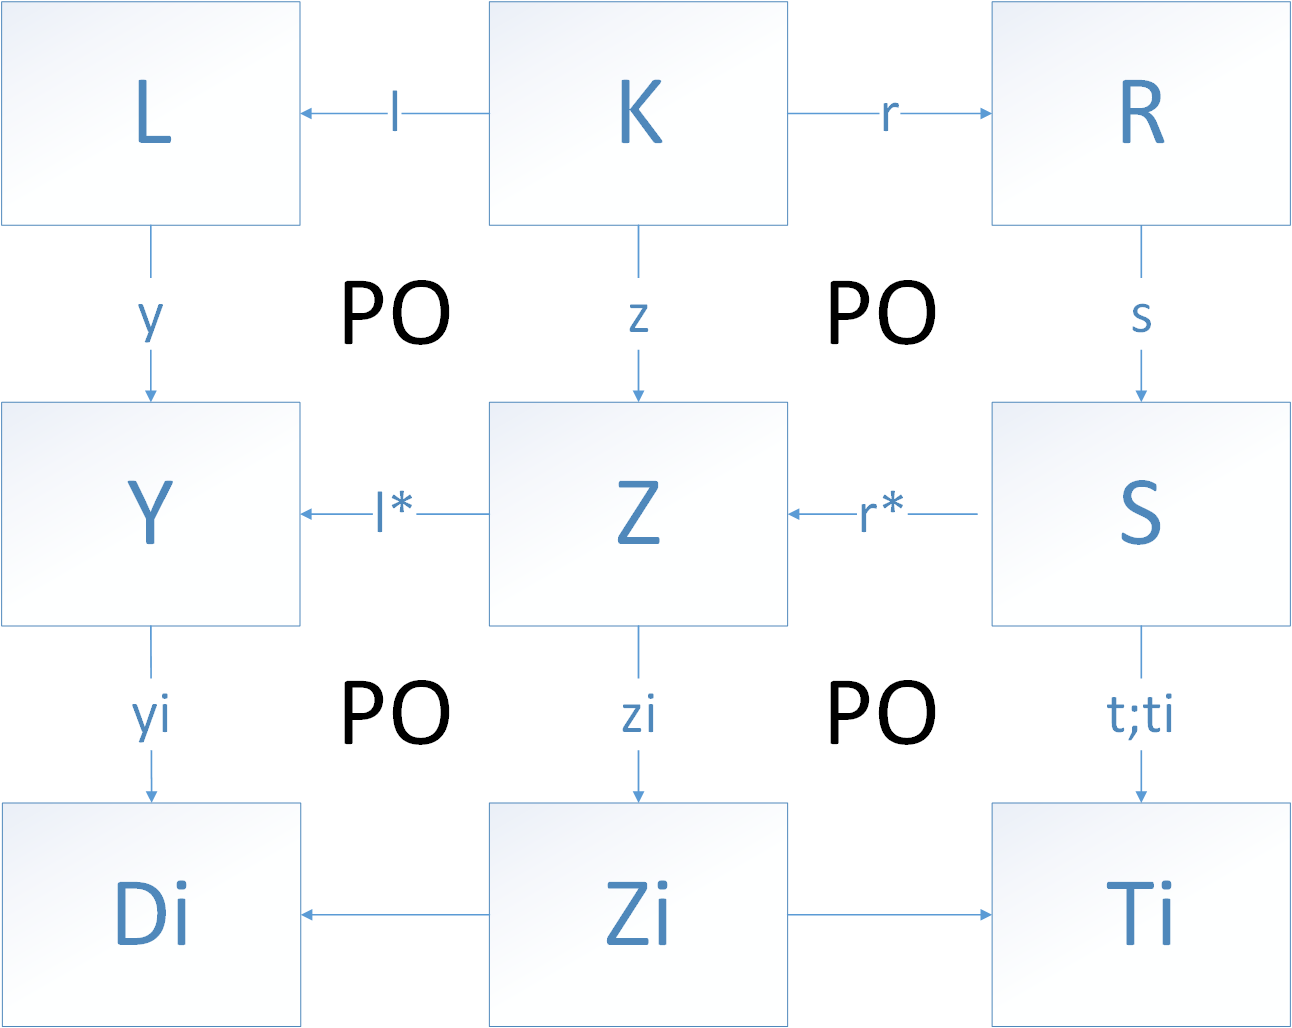
\includegraphics[height=.8\textheight]{Images/50_RightAC-To-LeftAC_Schema}
	\end{frame}
	
	\begin{frame}
		\frametitle{Construction of Left from Right Application Conditions}
		\framesubtitle{Construct pushout complement $Z$ -- Example}
		\centering
		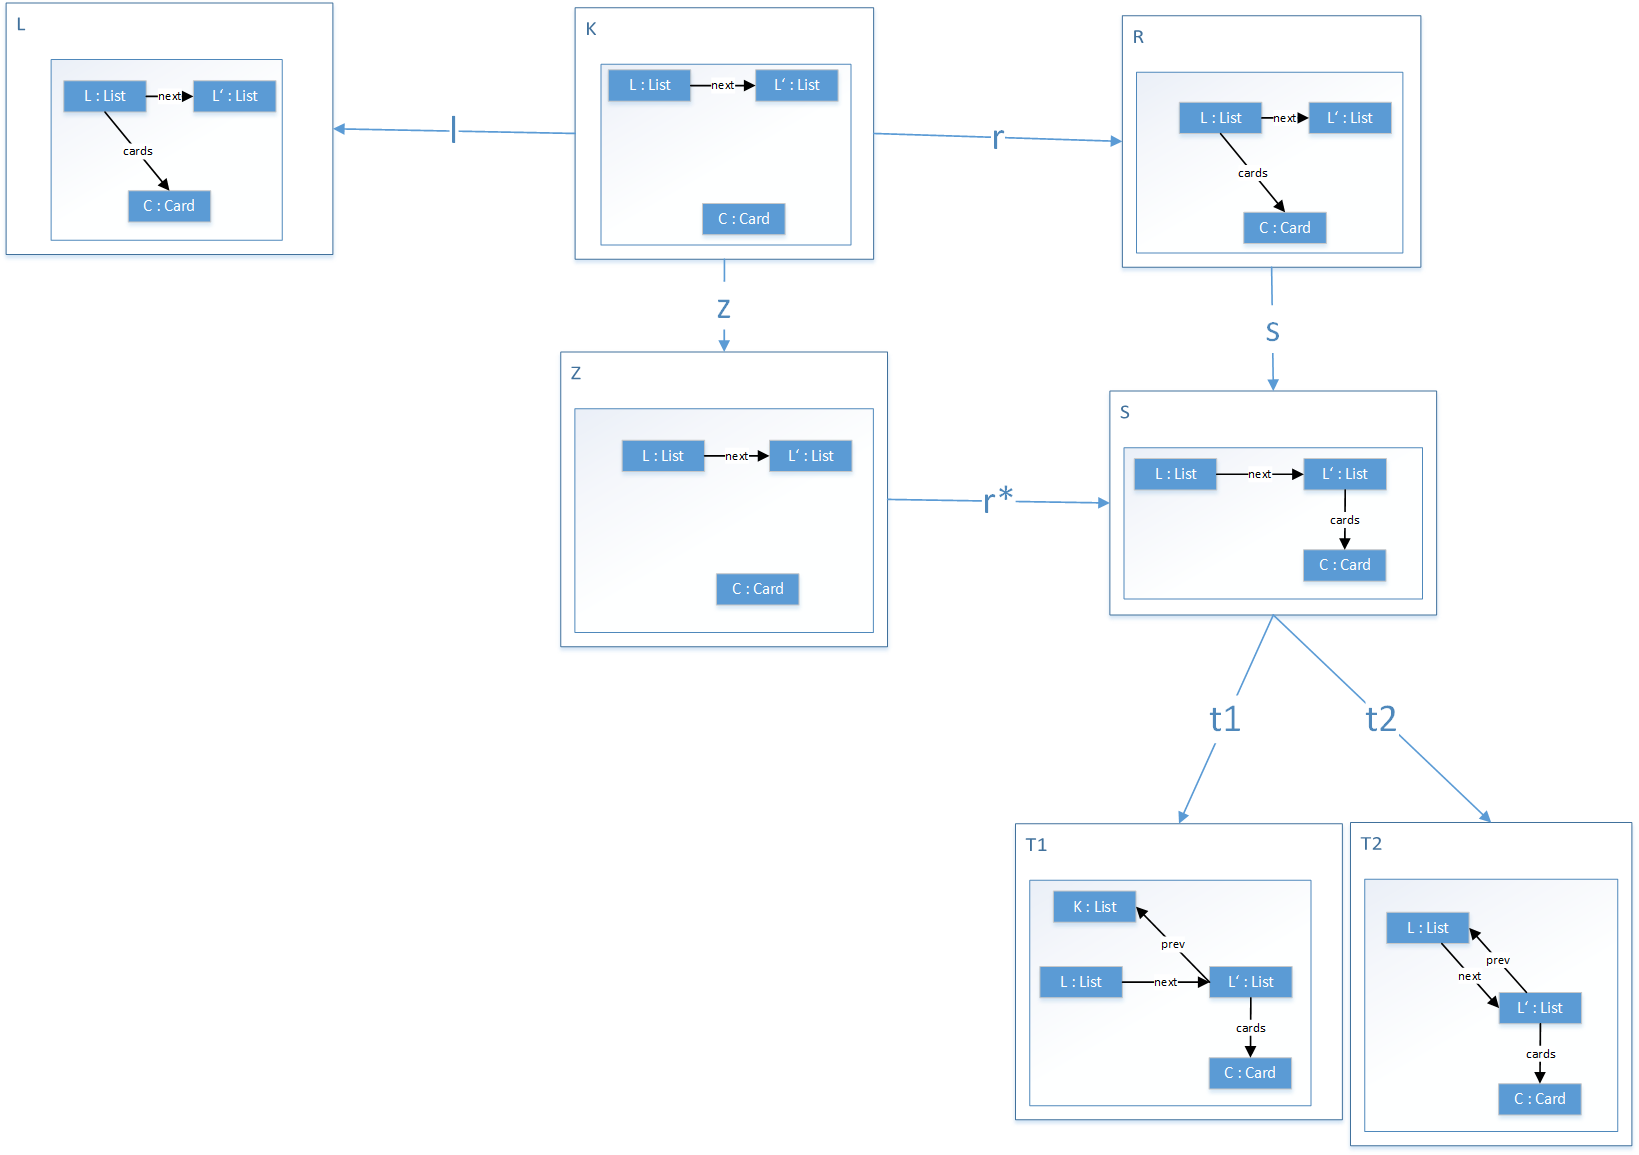
\includegraphics[height=.8\textheight]{Images/52_RightAC-To-LeftAC_Example_Step2}
	\end{frame}

	\begin{frame}
		\frametitle{Construction of Left from Right Application Conditions}
		\framesubtitle{Construct pushout $Y$ -- Example}
		\centering
		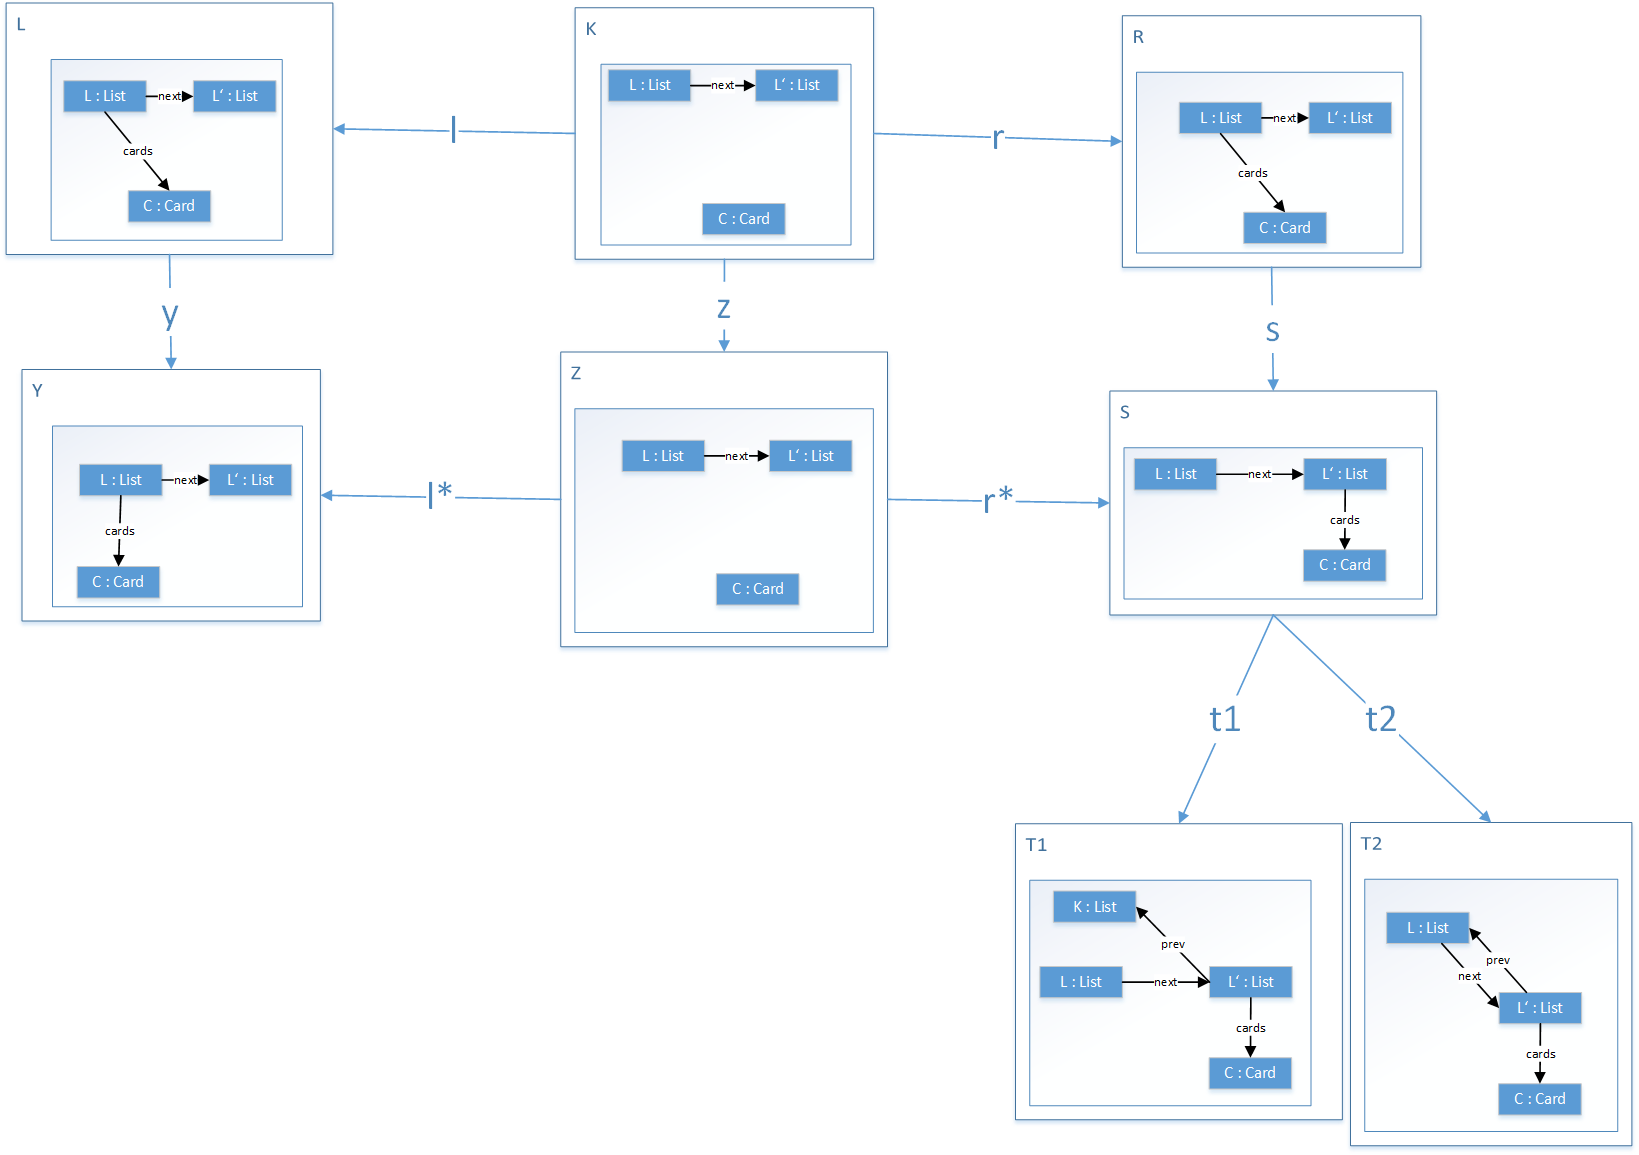
\includegraphics[height=.8\textheight]{Images/53_RightAC-To-LeftAC_Example_Step3}
	\end{frame}

	\begin{frame}
		\frametitle{Construction of Left from Right Application Conditions}
		\framesubtitle{Construct pushout complements $Z_i$ -- Example}
		\centering
		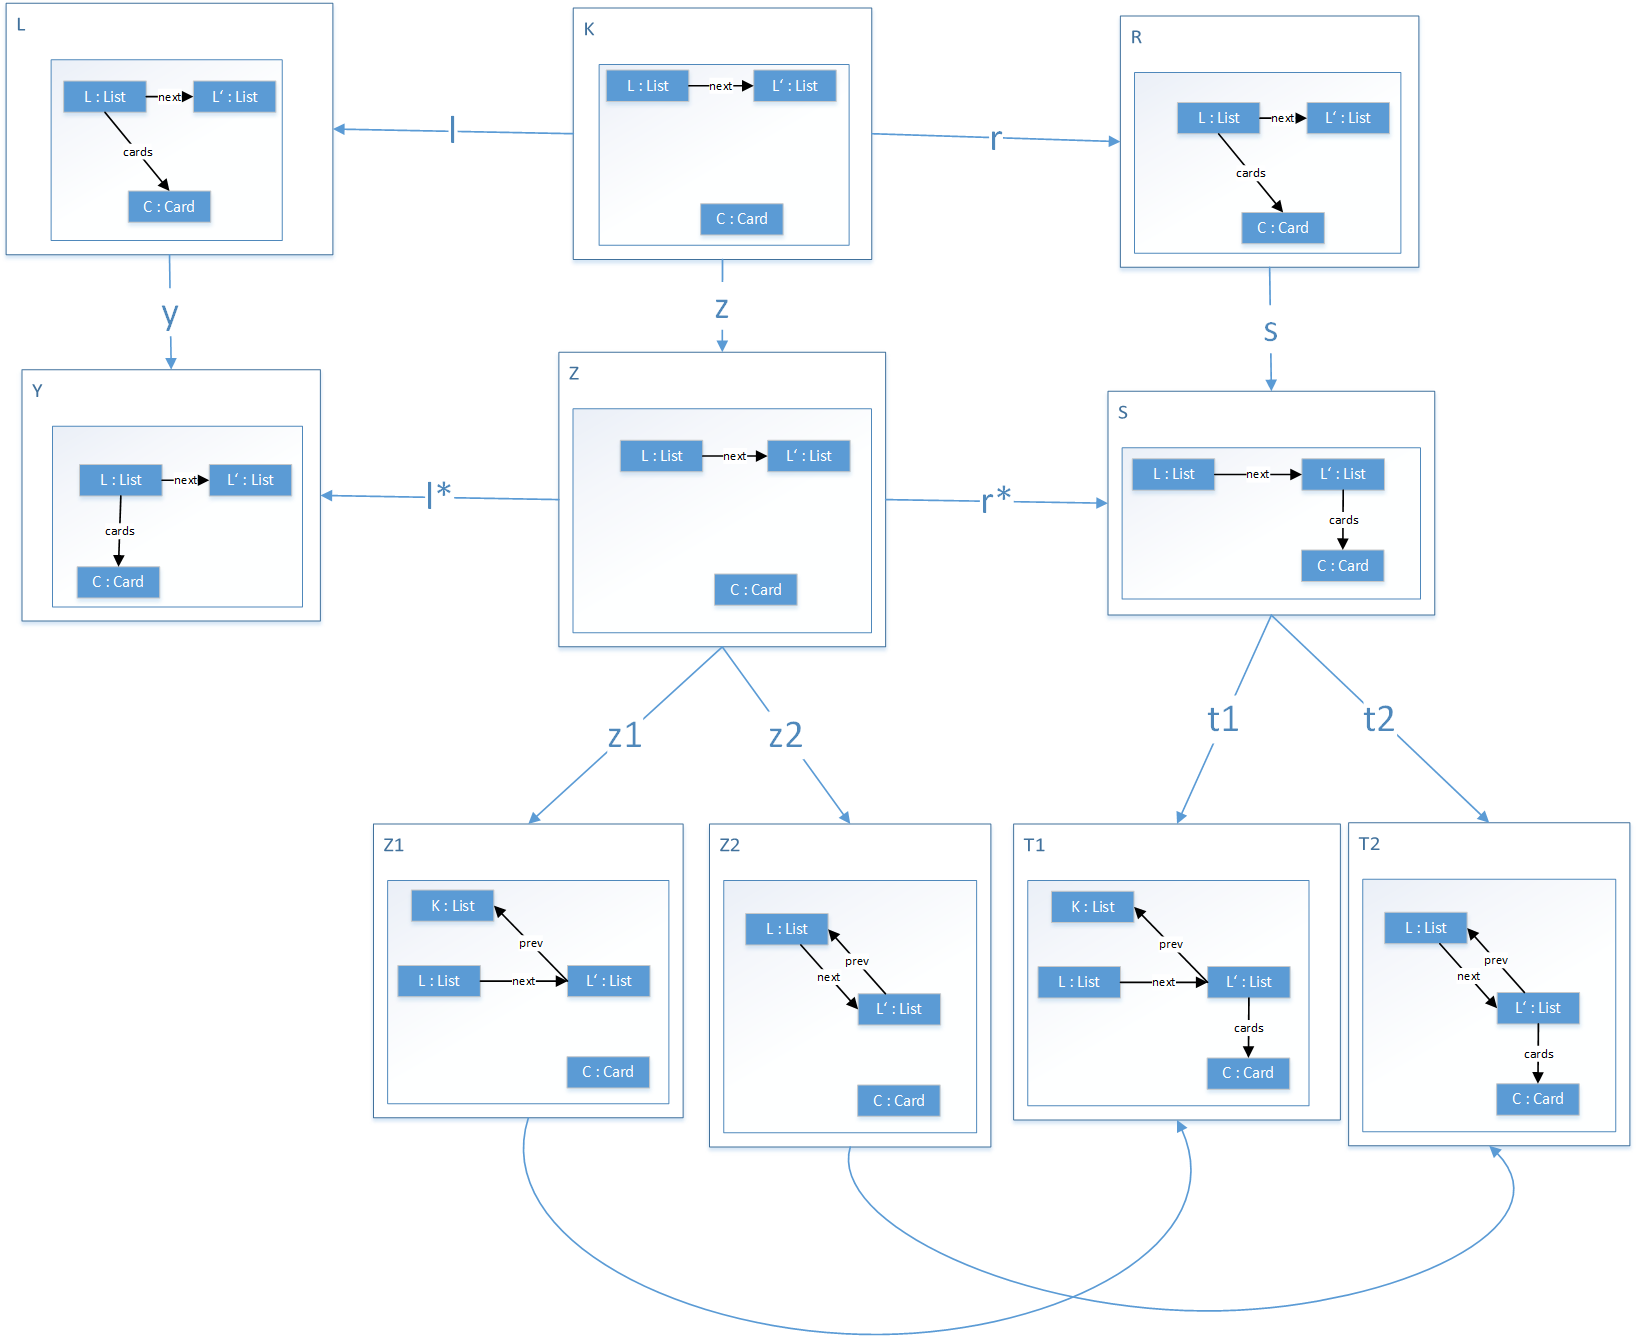
\includegraphics[height=.8\textheight]{Images/54_RightAC-To-LeftAC_Example_Step4}
	\end{frame}

	\begin{frame}
		\frametitle{Construction of Left from Right Application Conditions}
		\framesubtitle{Construct pushout $D_i$ -- Example}
		\centering
		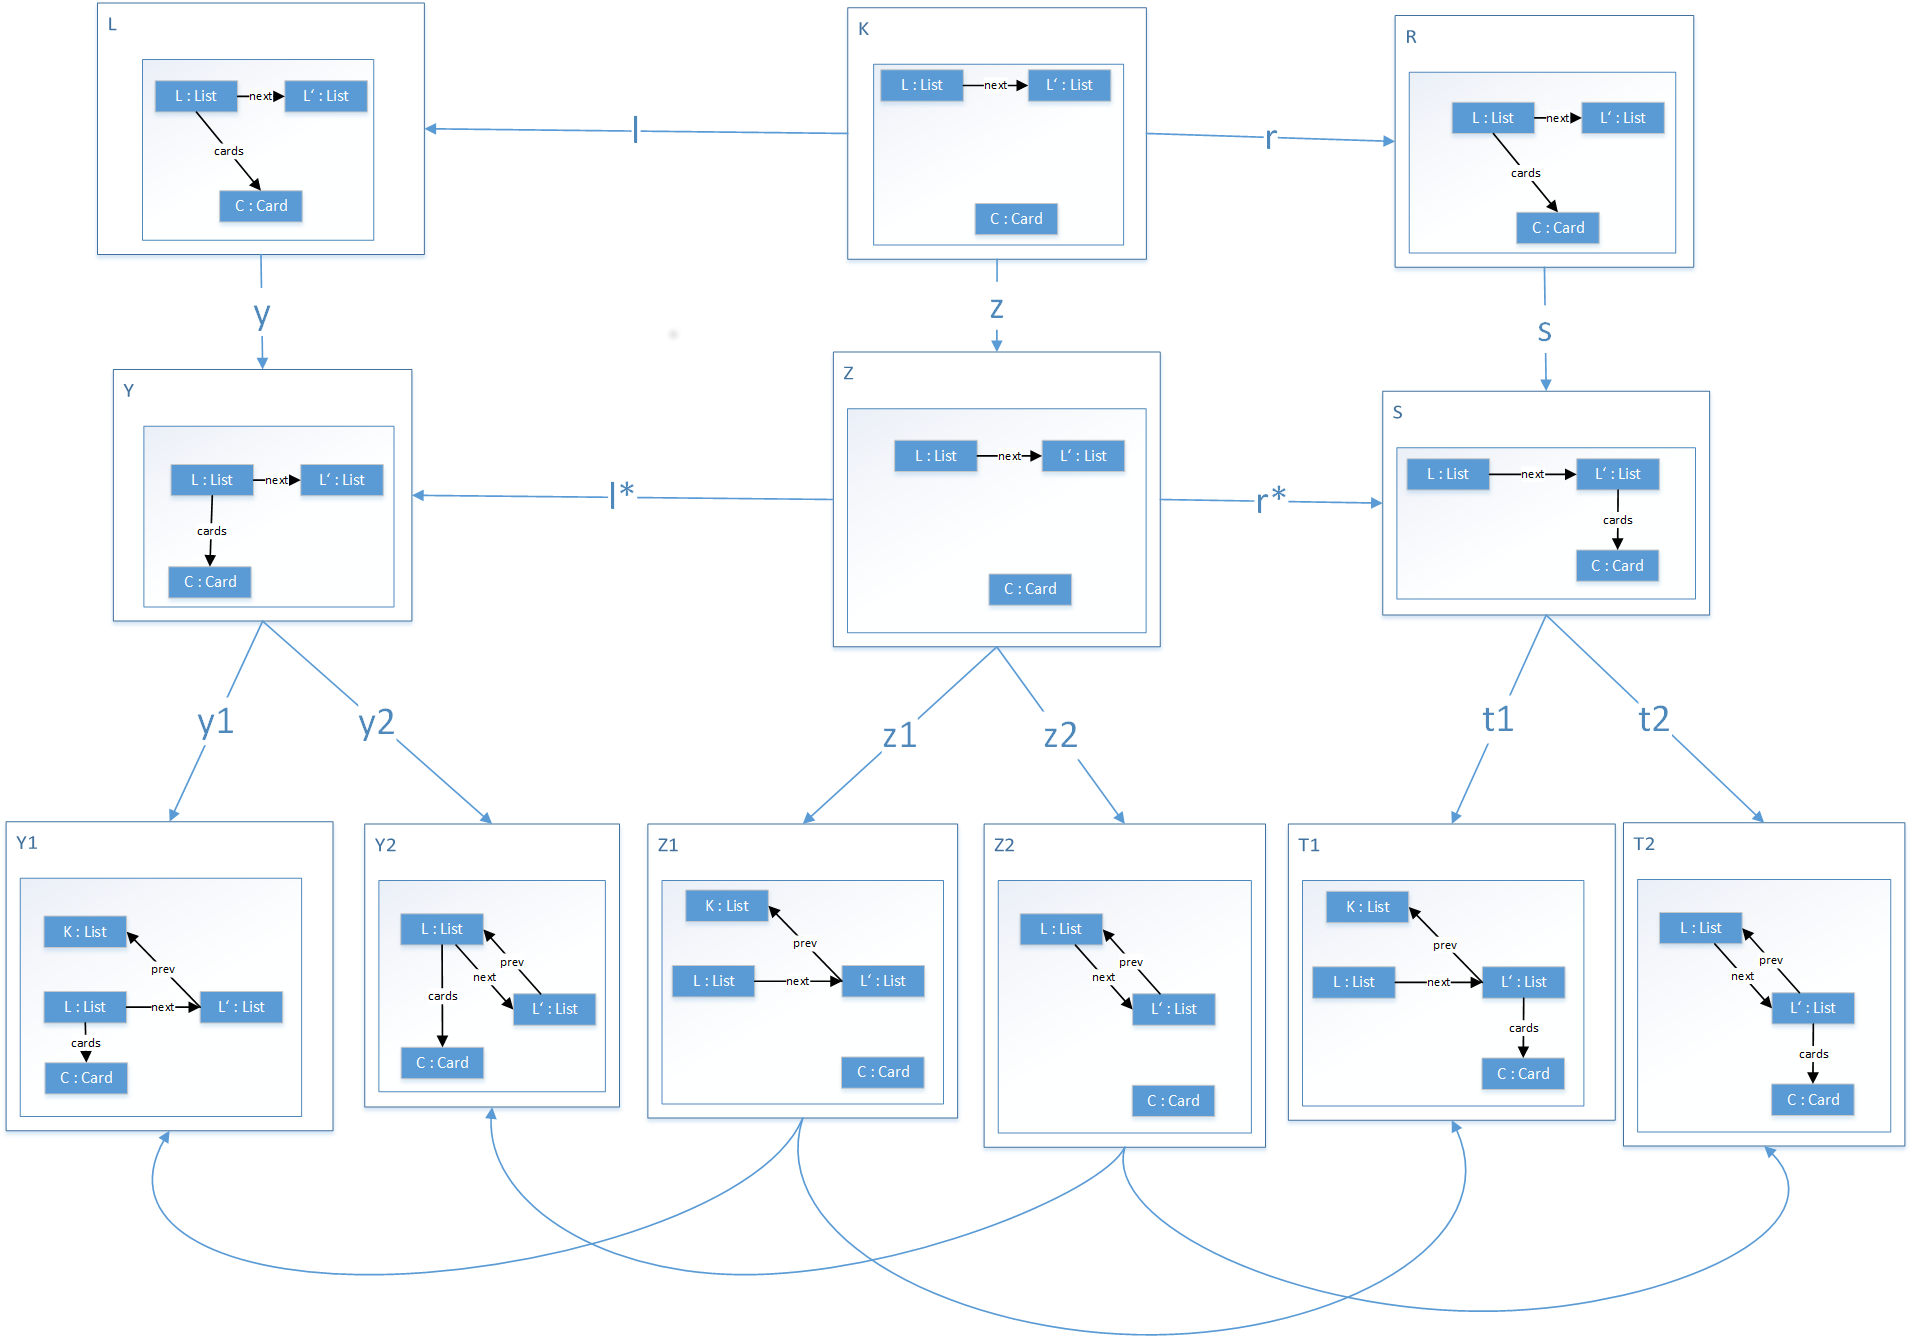
\includegraphics[height=.8\textheight]{Images/55_RightAC-To-LeftAC_Example_Step5}
	\end{frame}

	\begin{frame}
		\frametitle{Construction of Left from Right Application Conditions}
		\framesubtitle{Left Application Condition -- Example}
		\centering
		\includegraphics[width=\linewidth]{Images/60_Result-LeftAC}
	\end{frame}

	\begin{frame}
		\frametitle{Rule Application allowed?}
		\framesubtitle{Rule Example: Moving Card $C$ from List $L$ to $L'$}
		\centering
		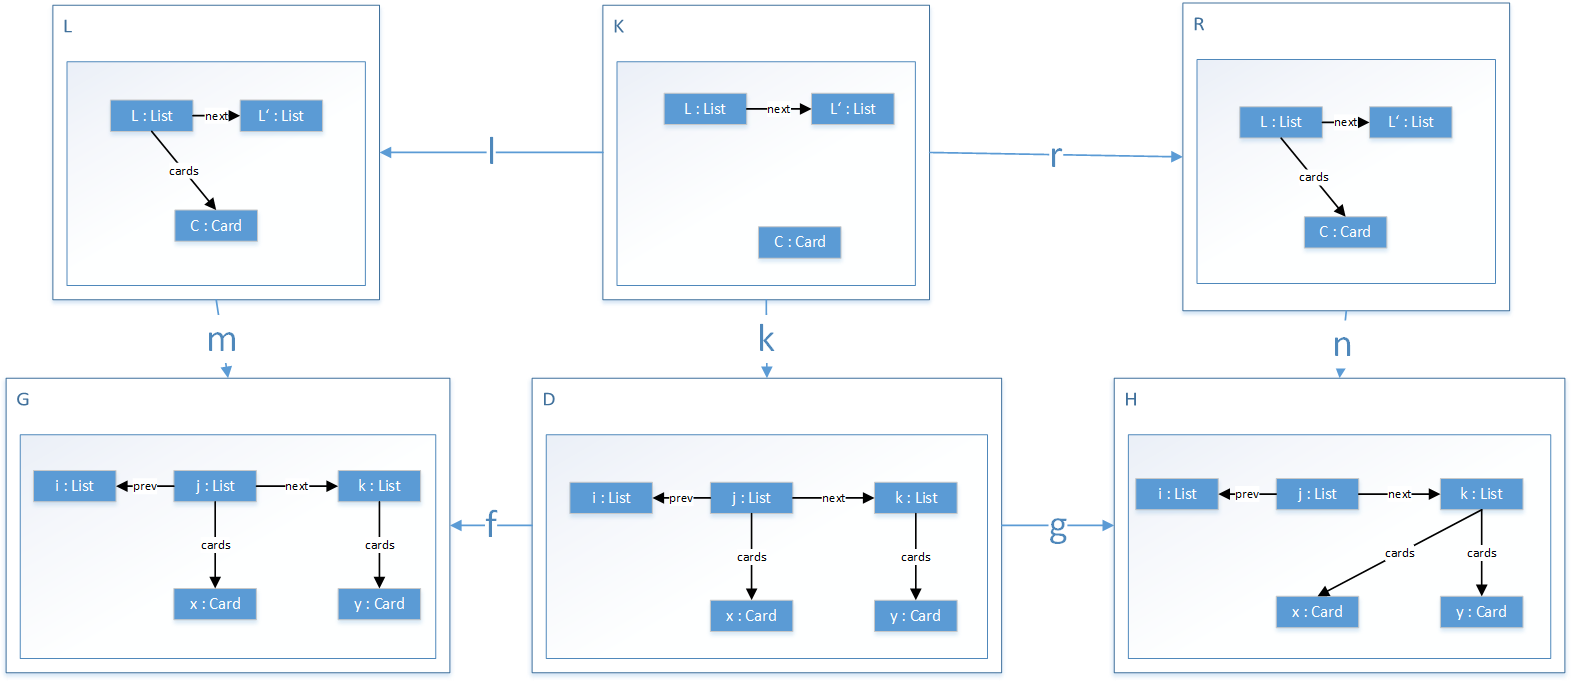
\includegraphics[width=\linewidth]{Images/01_Rule_Example}
	\end{frame}

\section{Conclusion}
	\begin{frame}
		\frametitle{Contents}
		\tableofcontents[currentsection]
	\end{frame}
	
	\begin{frame}
		\frametitle{Conclusion}
		\framesubtitle{}
		\begin{block}{Our implementation}
			\begin{itemize}
				\item interesting topic, worth repeating with focus on current performance limitations on larger examples
				\item The construction of application conditions can be implemented with the code from the exercises
				\begin{itemize}
					\item currently only implemented for constraint $c: P \rightarrow C$ (not multiple conclusions)
				\end{itemize}
			\end{itemize}
		\end{block}
	
		\begin{block}{Problems during implementation}
			\begin{itemize}
				\item difficult to output diagrams in PlantUML as labels are used to identify objects in the diagrams (but there exist multiple objects with the same label) - only limited help for debugging
				\item choose left or right and first or second in corners/spans? (missing documentation!)
			\end{itemize}
			$\Rightarrow$ code generation from category diagrams would be great!
		\end{block}
	\end{frame}
	
	\begin{frame}
		\frametitle{Literature}
		\framesubtitle{}
		Hartmut Ehrig, Karsten Ehrig, Ulrike Prange, and Gabriele
		Taentzer: \\
		Fundamentals of Algebraic Graph Transformation. \\
		Monographs in Theoretical Computer Science. An EATCS
		Series. Springer, 2006. \\
		Sections 7.2 and 7.3 (pp. 156-164)
	\end{frame}
\end{document}
